\chapter{Lecture 23 - More Thermal Conductivity Models, Convection Intro \& Review}
\label{ch:ch23}
\section{Objectives}
The objectives of this lecture are:
\begin{enumerate}
\item discuss gap conductance
\item present cladding and oxide layer thermal conductivity models
\item provide a summary/review of familiar convective heat transfer correlations
\end{enumerate}
\begin{marginfigure}
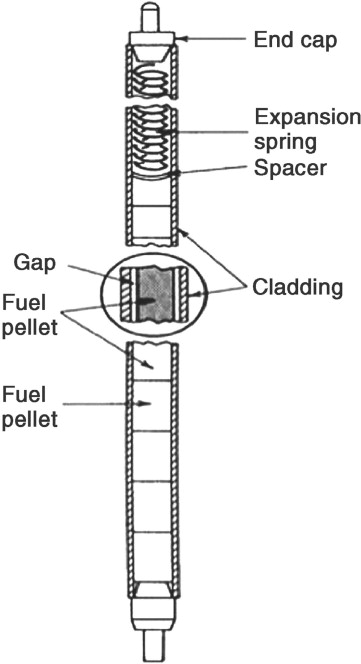
\includegraphics[width=2.5 cm]{pwr-fuel-pin.png}
\caption{Typical PWR fuel pin schematic.}
\label{fig:pwr-fuel-pin}
\end{marginfigure}
\section{Gap Conductance} \index{gap conductance}
Typical PWR fuel engineering results in a fuel pin comprising a stack of pellets within cladding.  The fuel pin is pressurized with an inert gas---typically helium--- and pellets are held in place axially with springs as illustrated in Figure \ref{fig:pwr-fuel-pin}.  Over time, multiple phenomena occur such as:\cite{bartel2015state}
\begin{enumerate}
\item fill gas composition changes due to production of fission product gasses
\item structural changes to the fuel pellet such as central void formation and  ``hourglassing'' due to sintering as illustrated in Figure \ref{fig:pellet_sinter}
\item ``creep-down'' of cladding in which the cladding deforms slowly---possibly coming into contact with the pellets---due to external coolant pressure at high material temperature.
\end{enumerate}

\begin{marginfigure}
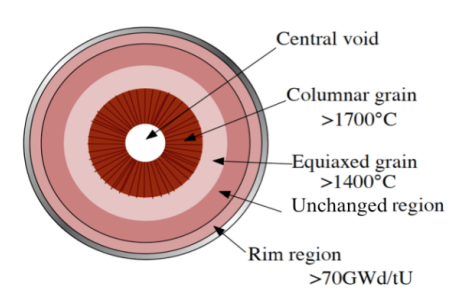
\includegraphics{sintered_pellet.png}
\caption{Schematic restructuring of nuclear fuel pellet after high temperature operation.}
\label{fig:pellet_sinter}
\end{marginfigure}

The void formation and complex structural re-alignment are most pronounced in fast reactor systems operating at very high temperature and high heat flux.  The aforementioned FRAPCON model captures the most important features that we will focus on in this course.  The gap conductance is the only other feature that we will include in this class.\sidenote{In order to capture all effects of re-structuring in the fuel pellet, different models would be needed for each region in the fuel.}  

For PWRs, the net dimensional changes can result in substantial contact between the fuel pellet and the cladding.  This actually improves thermal performance at the cost of increased risk of fuel pin failure due to clad rupture.  The mathematical model we have used for heat transfer across the fuel pellet to clad gap is:
\begin{equation}
\Delta T_{\text{gap}} = T_o - T_{ci} = \frac{q^{\prime}}{2 \pi r_g h_g}
\label{eq:gap_cond_ch23}
\end{equation}
where $h_g$ is the gap conductance.  But where does $h_g$ come from and how is it modeled?  For this course, we will consider gap conductance as a function of linear heat rate and of the initial cold diametrical gap.  Such a relationship is shown graphically in Figure \ref{fig:gap_cond}.  Note that as initial gap is reduced and as linear heat rate increases, the gap conductance increases. \marginnote{\textbf{Question:} Why would $h_g$ increase for higher values of $q^{\prime}$?} That will be the extent of our modeling of $h_g$ for this course.

\begin{marginfigure}
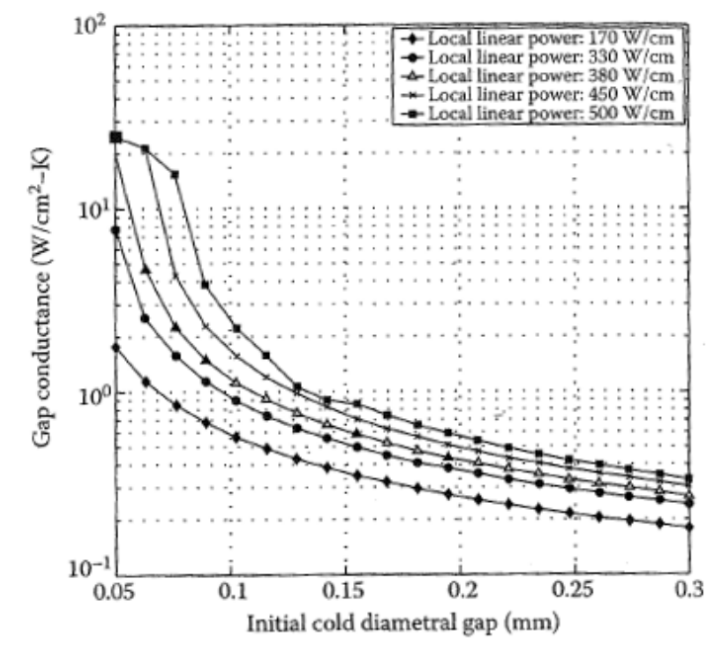
\includegraphics{gap_conductance.png}
\caption{Gap conductance as a function of linear heat rate and initial cold diametrical gap.}
\label{fig:gap_cond}
\end{marginfigure}


\section{Conduction through fuel cladding}
For Zircaloy cladding, the thermal conductivity used by FRAPCON 3.5 is given by Equation \ref{eq:clad_cond}.

\begin{equation}
k_{\text{clad}} = 7.51 + 2.09 \times 10^{-2}T - 1.45 \times 10^{-5} T^2 + 7.67 \times 10^{-9} T^3\ \ \text{[W/m-K]}
\label{eq:clad_cond}
\end{equation}
for temperature, $T$, given in Kelvin.  Following a similar derivation as for conduction in the fuel, the heat equation in cylindrical coordinates\sidenote{With the usual assumptions of symmetry with respect to $\phi$ and axial heat conduction being negligible.} for conduction in the cladding with temperature-dependent thermal conductivity can be reduced to:

\begin{equation}
\int_{T(r_{co})}^{T(r_{ci})} \ k(T) \ dT = \frac{q^{\prime}}{2 \pi} \ln{\left(\frac{r_{co}}{r_{ci}} \right)}
\label{eq:clad_heat}
\end{equation}

There may be some circumstances where this problem can be posed and solved analytically; for this class, the default method of solving heat transfer problems of this type will be to use MATLAB.  The method is completely analogous to fuel thermal conductivity and will be left for homework exercises.

\section{Conduction through Clad Oxide Layer}
At risk of being repetitive, we can apply the same mathematical tools to capture temperature-dependent conductivity effects in the oxide layer that forms on the exterior of metallic fuel cladding.  
Oxide layer thickness is a function of operating history and water chemistry.  Typical thickness is near $20\times 10^{-6}$m.  For the model we will use, thermal conductivity of this oxide layer is only weakly dependent on temperature.  One conductivity model of the oxide layer on Zircaloy cladding reads as follows:

\begin{equation}
k_{\text{oxide}}=0.835 - 1.81 \times 10^{-4}T \ \  \text{W/m-K}
\label{eq:cond_oxide}
\end{equation}
where, as usual, the temperature ($T$) is given in Kelvin. Similar to cladding, the steady-state heat equation can be transformed into Equation \ref{eq:oxide_heat}.

\begin{equation}
\int_{T(r_{oo})}^{T(r_{co})} k(T) \ dT = \frac{q^{\prime}}{2 \pi}\ln{\left(\frac{r_{oo}}{r_{co}} \right)}
\label{eq:oxide_heat}
\end{equation}
where $r_{oo}$ is the outer radius of the oxide layer.

\section{Overall Conduction Through Fuel Pin}

Cumulatively we have elaborated on the thermal models for the fuel pellet, pellet-to-clad gap, cladding, and the oxide layer outside the cladding.  While will not take the time to generalize the mathematical analysis such that we could derive the full temperature profile such as is illustrated in Figure \ref{fig:pin_temp_profile}, we can solve for the temperature at the interfaces between each region and at the pellet center line.

\begin{marginfigure}
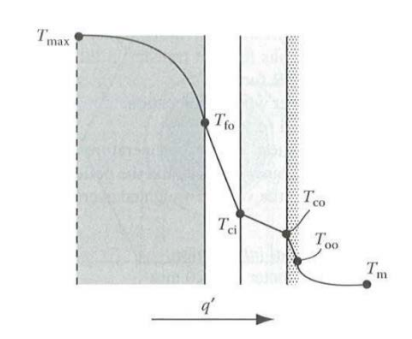
\includegraphics{fuel_pin_temp_profile.png}
\caption{Fuel pin temperature profile.}
\label{fig:pin_temp_profile}
\end{marginfigure}

\section{Convective Heat Transfer Correlations}
We have not yet elaborated on the analysis of heat transfer between the fuel clad (or fuel clad oxide) outer surface and the bulk coolant.  In elementary courses it may have sufficed for us to simply provide a convective heat transfer coefficient, $h_{\text{cool}}$, and plug the number into an equation to find $\Delta T_{\text{cool}}$.  In this course we will pick up where your heat transfer course left off and discuss a variety of heat transfer correlations relevant to convective heat transfer in nuclear applications.

\index{Nusselt number} 
\newthought{For non-metallic fluids} in fully developed turbulent flow, correlations for convective heat transfer are presented in the context of the non-dimensional Nusselt number.\marginnote{\textbf{Nusselt number:} relates to the temperature gradient at the wall of a fluid-solid interface and the overall temperature difference between the wall and the bulk fluid.}  The Nusselt number is a function of fluid material properties as well as the flow condition and is defined by Equation \ref{eq:nusselt}

\begin{equation}
\text{Nu} = \frac{h D}{k}
\label{eq:nusselt}
\end{equation}
where $h$ is the convective heat transfer coefficient, $D$ is a characteristic length like pipe diameter or hydraulic diameter, and $k$ is the fluid thermal conductivity.  The correlations developed are usually of the form shown in Equation \ref{eq:nusselt_corr_general}.

\begin{equation}
\text{Nu} = \text{C}\text{Re}^{\alpha}\text{Pr}^{\beta} \left(\frac{\mu_w}{\mu} \right)^{\kappa}
\label{eq:nusselt_corr_general}
\end{equation}  \index{Prandtl Number}
where $\text{Re}$ is the Reynolds number, $\text{Pr}$ is the Prandtl number of the fluid, $\mu$ and $\mu_w$ are the viscosity of the fluid in the bulk flow and along the wall where heat transfer takes place, respectively; and $C$,$\alpha$,$\beta$, and $\kappa$ are given constants.\marginnote{\textbf{Prandtl Number:} a dimensionless fluid property that describes the ratio of viscous diffusivity to thermal diffusivity.}

\section{Correlations for Circular Tubes}
Several correlations are available for convective heat transfer in circular tubes.
\subsection{Dittus-Boelter Correlation} \index{Dittus-Boelter}
This is a widely used correlation\cite[-2.5cm]{dittus1985heat} that we will present only for fully-developed turbulent flow.\sidenote[][-1.0cm]{As with the hydraulics analysis, we ignore heat transfer conditions near entrances or exits or, in short, anywhere other than ``fully-developed'' regions where the flow-field is undisturbed by such effects. Generally speaking convective heat transfer is enhanced in entrance regions owing to the increased ``action'' in the fluid flow field.} The correlation is given by Equation \ref{eq:dittus-boelter}.

\begin{equation}
\text{Nu}_{\infty} = 0.023 \text{Re}^{0.8}\text{Pr}^{0.4}
\label{eq:dittus-boelter}
\end{equation}\marginnote[0.5cm]{\textbf{Note:} The $\infty$ subscript in $\text{Nu}_{\infty}$ is meant to denote that the correlation is valid for a location ``infinitely far'' from any entrance, exit, discontinuity, or other feature that would disrupt the fully developed turbulent flow.  We will read $\infty$ simply to imply fully developed flow.}  The following limits apply to the Dittus-Boelter correlation: 

\begin{equation*}
\text{Re}>10,000\text{,  }0.7 < \text{Pr} < 100\text{, and }\sfrac{L}{D}>60;
\end{equation*} 
where $L$ corresponds to position along a circular tube and $D$ is the tube diameter.

\subsection{Colburn Correlation} \index{Colburn}
For fluids with high viscosity consider the Colburn correlation.\cite{colburn1964method}
\begin{equation}
\text{St}\text{Pr}=0.023 \text{Re}^{-0.2}
\label{eq:colburn}
\end{equation}
which, despite the note that this should be used with high viscosity fluids, has the same range of applicability as the Dittus-Boelter correlation.  The Stanton Number ($\text{St}$) combines the Nusselt number, Reynolds number, and Prandtl number and is given by:\marginnote{\textbf{Stanton Number:} a dimensionless fluid property that characterizes the ratio of heat transfer at the wall to the energy transported by the fluid flow stream.} \index{Stanton number}
\begin{equation}
\text{St} = \frac{\text{Nu}}{\text{Re}\text{Pr}}
\label{eq:stanton}
\end{equation}

Applying Equation \ref{eq:stanton}, then Equation \ref{eq:colburn} becomes:
\begin{equation}
\text{Nu}_{\infty} = 0.023 \text{Re}^{0.8}\text{Pr}^{\sfrac{1}{3}}
\end{equation}

\subsection{Seider and Tate Correlations} \index{Seider and Tate}
This correlation\cite{sieder1936heat} is suitable for diabetic flows of fluids including organic liquids, petroleum fractions, and air.  

For organic liquids:

\begin{equation}
\text{Nu}_{\infty} = 0.015 \text{Re}^{0.85} \text{Pr}^{0.3}
\label{eq:st-organic}
\end{equation}

For petroleum fractions:
\begin{equation}
\text{Nu}_{\infty} = 0.027 \text{Re}^{0.8}\text{Pr}^{\sfrac{1}{3}}\left(\frac{\mu_w}{\mu} \right)^{-0.14}
\label{eq:st-petroleum}
\end{equation}

For air:
\begin{equation}
\text{Nu}_{\infty} = 0.023 \text{Re}^{0.8}\text{Pr}^{\sfrac{1}{3}}\left(\frac{\mu_w}{\mu} \right)^{-0.14}
\label{eq:st-air}
\end{equation}
where for Equation \ref{eq:st-petroleum} and \ref{eq:st-air} all material properties should be evaluated at the bulk condition except, of course, $\mu_w$ which should be evaluated at the prevailing temperature and pressure along the wall.  The range of applicability of the Seider and Tate correlations will be taken to be the same as those for the Dittus-Boelter correlation.

\subsection{Gnielinski Correlations} \index{Gnielinski}
A more recent correlation\cite{gnielinski1976new} is available that extends previous work and covers transitionally turbulent flows. 

For liquids:
\begin{equation}
\text{Nu}_{\infty} = 0.0120\left(\text{Re}^{0.87}-280 \right)\text{Pr}^{0.4}
\label{eq:gniel-liquid}
\end{equation}
where $0.4 < \text{Pr} < 1.5,$ and $2300 < \text{Re} < 5 \times 10^6$.

For gases:
\begin{equation}
\text{Nu}_{\infty} = 0.0214\left(\text{Re}^{0.80}-100 \right)\text{Pr}^{0.4}
\label{eq:gniel-gas}
\end{equation}
where $1.5 < \text{Pr} < 500$, and $2300 < \text{Re} < 5 \times 10^6$.

\subsection{Diabetic flow} 
In cases where heating and cooling of the fluid result in significant variation in the physical properties, one should use the correlations due to Gnielinski which is an extension of the Petukhov correlation that we used in our hydraulic analysis.  In this case, the basic Nusselt number will be calculated as:

\begin{equation}
\text{Nu}_{D} = \frac{\left(\sfrac{f}{8}\right)(\text{Re} - 1000)\text{Pr}}{1+12.7\sqrt{\sfrac{f}{8}}\left(\text{Pr}^{\sfrac{2}{3}}-1 \right)}
\label{eq:petukhov}
\end{equation}
where $f$ is given by:
\begin{equation}
f = \left(1.82 \log_{10}{\text{Re}} - 1.64 \right)^{-2}
\end{equation}

Once this Nusselt number has been determined, as with friction factors in the hydraulics section of the course, we modify the Nusselt number to take into account the variability in fluid properties between the bulk conditions and those that prevail along the wall where heat transfer occurs.

For liquids:
\begin{equation}
\frac{\text{Nu}}{\text{Nu}_{D}} = \left(\frac{\mu_b}{\mu_w} \right)^{m}
\end{equation}

For gases:
\begin{equation}
\frac{\text{Nu}}{\text{Nu}_{D}} = \left(\frac{T_b}{T_w} \right)^{m}
\end{equation}

The coefficient $m$ for corresponding conditions is provided in Table \ref{tab:Pet}
\begin{table}
\begin{tabular}{l c c}
\toprule
  &  \textbf{Liquids} & \textbf{Gases} \\
  &  \boldmath{$0.025 \le \sfrac{\mu_b}{\mu_w} \le 12.5$} & \boldmath{$0.27 \le \sfrac{T_b}{T_w} \le 2.7 $}\\
\hline
Heating $(T_w > T_b)$ & m = 0.11 & m = 0.47 \\
Cooling $(T_w < T_b)$ & m = 0.25 & m = 0 \\
\bottomrule
\end{tabular}
\caption{Exponent for Petukhov correlation.}
\label{tab:Pet}
\end{table}
